\begin{multicols}{3}[\section{UMA}]

\rhead{Daniel Keilmann}
\lfoot{13.05.2016}

\newrefsegment

\begin{tabular}{p{2,1 cm}p{2.7 cm}}
\textbf{Steckbrief}& \\
\end{tabular}
\rowcolors{1}{\topicolor!20}{}
\begin{tabular}{p{2,1 cm}p{2.7 cm}}
      Einsatz seit & 2004\\
      Verbreitung & USA, CA, FR, GB\\
	  Einführung in Deutschland & 2006\\
      Eingestellt in Deutschland & 2006 (kurz nach Einführung)\\
	  Standards & UMA-Standard\\
\end{tabular}
\par
\subsection*{Überblick}
Der Kommunikationsstandard UMA (\textbf{U}nlicensed \textbf{M}obile \textbf{A}ccess) ermöglicht es GSM-, GPRS/EDGE- und UMTS/HSDPA-Dienste über Bluetooth oder WLAN-Dienste im lizenzfreien Frequenzband ISM zu realisieren.\\	
Unlicensed (unlizenziert) heißt in diesem Zusammenhang, dass weder der Mobilfunkkunde noch der Netzbetreiber Lizenzen für den Betrieb zahlen muss. Im Gegensatz dazu, fallen im klassischen Mobilfunk Kosten an. UMA ist nicht eine einfache VoIP Verbindung über WLAN bzw. Bluetooth (VoWLAN), sondern der Standard erlaubt auch Handover und Roaming, also die Übernahme von laufenden Gesprächen.~\cite{uma.3}
Es benutzt Wi-Fi (802.11b/g) um Handys mit dem Internet zu verbinden. UMA ist mit einem Dual-Mode-Handy erreichbar.~\cite{uma.1}

\subsection*{Technische Erläuterung}
Wenn ein UMA fähiges Mobiltelefon in Reichweite von einem Wi-Fi-Netz kommt, stellt es eine Verbindung zu dem Router (WR) her, um Zugriff zum Internet zu erlangen. Nach erfolgreichem Verbinden mit dem Internet \enquote{eröffnet} das Mobilfunkgerät einen abgesicherten Tunnel zum Netzwerk von \textit{T-Mobile} (Security Gateway). Ist der Benutzer angemeldet und autorisiert für die UMA Benutzung, dann hat das Mobiltelefon über den UNC (\textbf{U}MA \textbf{N}etwork \textbf{C}ontroller) eine erfolgreiche Verbindung zum Netzwerk von \textit{T-Mobile} hergestellt und ist bereit auf Anfragen zu reagieren.~\cite{uma.1}

\subsection*{Vergleich UMA und GSM}
Der Unterschied zwischen einer UMA und einer GSM Verbindung liegt darin, dass UMA Mobilfunkanrufe nicht über einen GSM Funkturm weiterleitet. Dies wird realisiert indem das Handy eine virtuelle GSM Verbindung über das Internet herstellt. Durch das Herstellen einer Verbindung über das Internet und nicht durch die Funktürme, können Netzwerküberlastungen und Kapazitäten bedingte Probleme besser verhindert werden.~\cite{uma.1}

\subsection*{Übergang von UMA zum GAN}
Die ersten UMA Spezifikationen (R1.0.0.) wurden im September 2004 veröffentlicht. Nach dieser Erstveröffentlichung wurden diese UMA Spezifikationen der \textit{3GPP} (\textbf{3}rd \textbf{G}eneration \textbf{P}artnership \textbf{P}roject) Organisation, als Teil des \textit{3GPP} Themas „Generic Access to A/Gb interfaces“, übergeben. 
Am 8. April 2005 genehmigte die Leitung des \textit{3GPP} die Aufnahme der Spezifikation für „Generic Access to A/Gb interfaces“ in das \textit{3GPP} Release 6 (3GPP TS 43.318). 
Bei der Übergabe an \textit{3GPP} wurden gegenüber den Spezifikationen des UMA Protokoll und der UMA Architektur nur triviale Änderungen in der Terminologie vorgenommen.
Was vorher als UMA bezeichnet wurde, heißt unter \textit{3GPP} nun \textit{Generic Access Network} oder \textit{GAN}. Der UMA Network Controller wird nunmehr als Generic Access Network Controller oder GANC bezeichnet.
\begin{Figure}
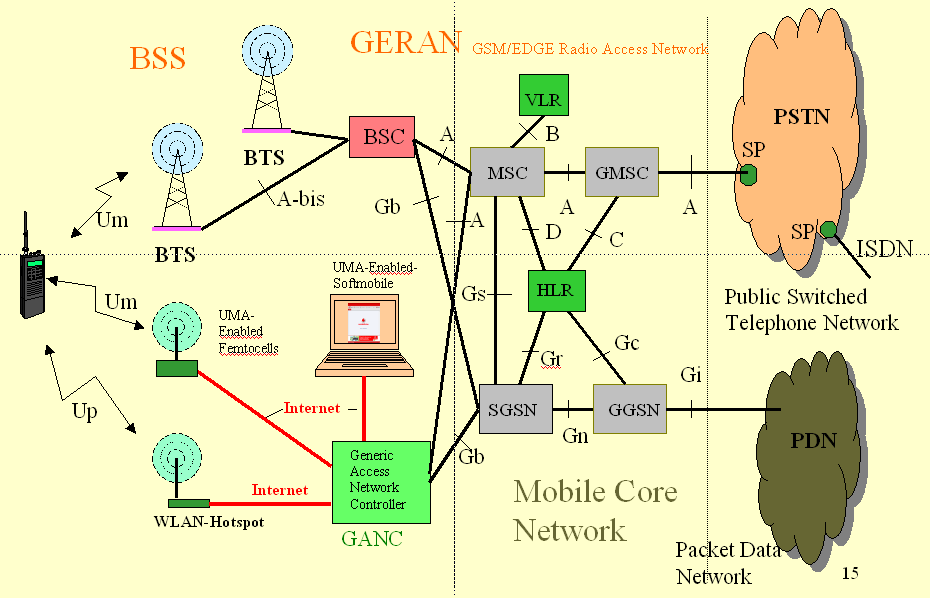
\includegraphics[width=\linewidth]{Kapitel/UMA/Grafiken/GANC_Rolle.png}
\captionof{figure}{GANC Rolle~\cite{uma.4}}
\label{fig:uma.GANC_Rolle}
\end{Figure}
Wie aus Abb. \ref{fig:uma.GANC_Rolle} hervorgeht, spielt der GANC offenbar die Rolle des BSC im GERAN. Während der Base Station Controller über das A-bis Interface mit den BTS verbunden ist, existieren drei Varianten der Anbindung des GANC an die Nutzerumgebung.\\
Variante 1 besteht in der Verwendung eines Mobiltelefons, das außer dem GSM-Betriebssystem noch eine Wi-Fi Komponente enthält. Das Interface mit dem
das Mobiltelefon über die Luftschnittstelle kommuniziert wird als Um-Interface bezeichnet. Die Wi-Fi Komponente gestattet über einen WLAN-Hotspot und das Internet mit dem GANC und damit mit dem Mobile Core Network Verbindung aufzunehmen. Dies nennt man Up-Interface.\\
Variante 2 sieht die Einrichtung einer Mini-BTS vor. Mit einer derartigen Femto-Cells genannten Einrichtung stellen Unternehmen eigene UMTS-Zugangspunkte als Internet-Access-Points bereit, über die Daten mit normalen Mobiles gesendet und empfangen werden können.\\
Variante 3 wird durch einen PC gebildet, auf dem ein UMA/GAN-taugliches Softmobile installiert ist, mit dem über das Internet und das Mobilfunknetz kommuniziert werden kann.\\
In allen drei Fällen stellt der GANC eine Brücke zwischen Wi-Fi und Cellular-Network dar. Eine Besonderheit gegenüber dem BSC besteht darin, dass der GANC ein SEGW (\textbf{Se}curity \textbf{G}ate\textbf{w}ay) enthält, das den Abschluss eines secure remote access tunnels zur Mobilstation bildet. Der Tunnel gestattet wechselseitige Authentication, Verschlüsselung und garantiert Datenintegrität sowohl für Signalisierung als auch für Sprach und Daten-Verkehr.
\begin{Figure}
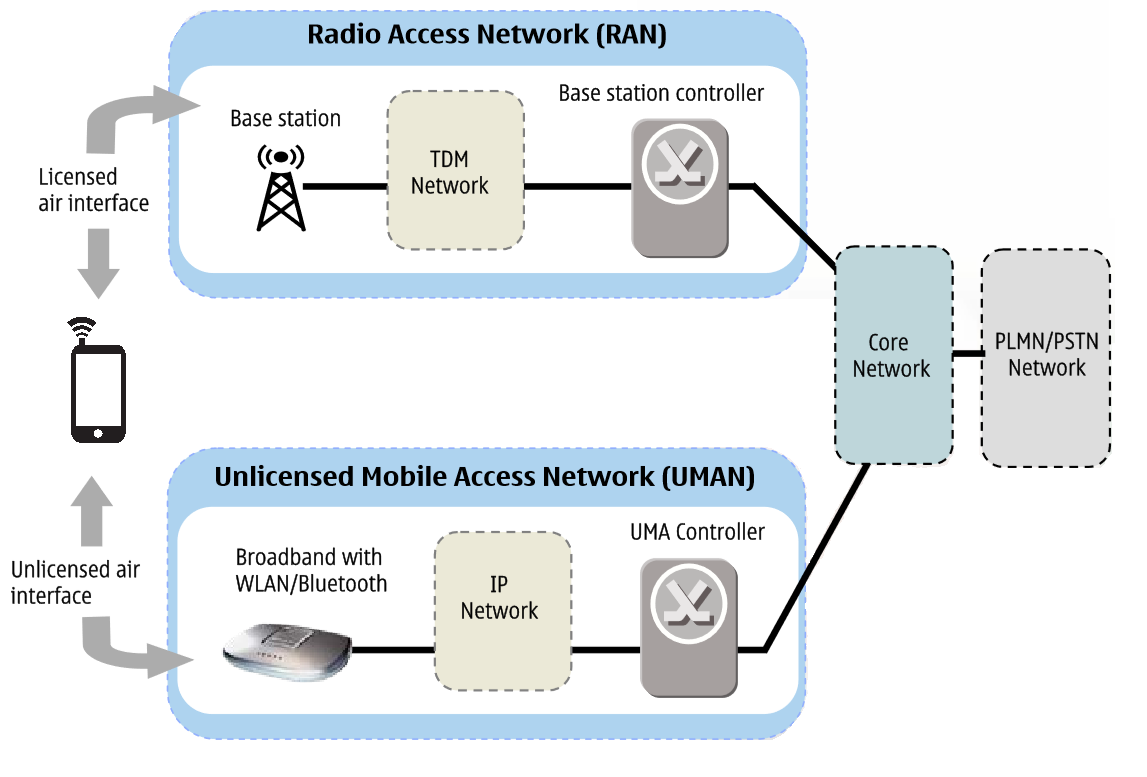
\includegraphics[width=\linewidth]{Kapitel/UMA/Grafiken/UMAN.png}
\captionof{figure}{UMA Network~\cite{uma.17}}
\label{fig:uma.UMAN}
\end{Figure}
\subsection*{Einsatz}
Vorteile von UMA für die 
Anwender:
\begin{itemize}
	\item Das betreiben eines Mobiltelefons ist an vielen Orten und über verschiedene Netzwerke möglich, aber man benötigt nur eine Rufnummer. 
	\item Benutzer können ihr WLAN selber einrichten, somit können Funklöcher des Anbieters überbrückt werden.
	\item Roaming (Nutzen des Mobiltelefons außerhalb des eigenen Mobilfunknetzes) verursacht keine Kosten mehr, weil Verbindungen mit öffent-lichen unlizenzierten WLANs möglich ist.
   	\item Anrufe über das Mobiltelefon werden zuverlässiger und kostengünstiger.~\cite{uma.2}
\end{itemize}
Anbieter: 
\begin{itemize}
	\item Betreiber können Wi-Fi Hotspots zur Verfügung stellen, wenn das Funknetz nicht ausreicht. 
	\item Überlastung des GSM und andere WLAN Netzwerke werden entlastet (Abgabe an WLANs).
	\item Wi-Fi eignet sich mehr für andere Übertragungsmedien als die Sprache.
	\item UMA befindet sich in der IP Netzwerk Schicht im ProtokollStack, dadurch ist es für viele Protokolle in der Interface Schicht verfügbar. Also ist UMA nicht auf ein Netzwerk beschränkt (Wi-Fi, Bluetooth etc.)~\cite{uma.2}
\end{itemize}
Nachteile von UMA:
\begin{itemize}
	\item Mobiltelefone müssen UMA kompatibel sein, was selten und teuer ist. Dies ist ein Problem für den Anbieter und Benutzer.
	\item UMA bietet Mobilität an, aber es kann keine kostenlose oder sehr günstige Kosten durch das Telefonieren ermöglichen. Es können keine SIP-basierten Dienste, wie Skype, verwendet werden.~\cite{uma.2}
\end{itemize}

\subsection*{Anbieter und Gremien}
Einsatzort des UMA ist insbesondere in den USA, Frankreich, Kanada und England. Dort ist der Dienst auch ein großer Erfolg. In Deutschland wurde UMA 2006 eingeführt, dies entsprach aber nicht dem UMA-Standard und unterstützte nicht die Funktion des Handover oder EAP-Sim. \enquote{EAP (\textbf{E}xtensible \textbf{A}uthentication \textbf{P}rotocol) ist ein von der IETF (\textbf{I}nternet \textbf{E}ngineering \textbf{T}ask \textbf{F}orce) entwickeltes, allgemeines Authentifizierungsprotokoll, das unterschiedliche Authentisierungsverfahren unterstützt, wie z. B. Username/Password, Digitales Zertifikat, SIM-Karte. EAP wird oft für die Zugriffskontrolle in WLANs genutzt.}~\cite{uma.13} Durch die EAP-SIM Methode erfolgt das Einklinken in ein verschlüsseltes WLAN automatisch. Dies wird dadurch realisiert, dass der Client (=Mobiltelefon) sich im Triple-A-System durch seinen SIM-Authentifizierungs-Algorithmus einwählt und somit die Eingabe eines voreingestellten WLAN-Passworts nicht benötigt wird.~\cite{uma.13} 
Außerdem wurde UMA in Deutschland nur mithilfe von einem Handset für die Telekom verfügbar, welches fehleranfällig war. Somit wurde es nach wenigen Monaten wieder eingestellt.\\
Ein weiterer Vorteil von dem UMA-Standard ist die weitflächige Unterstützung der Gerätehersteller:
\begin{itemize}
	\item \textit{LG}
	\item \textit{RIM/Blackberry}
	\item \textit{Nokia}
	\item \textit{Samsung}
	\item \textit{Motorola}
	\item \textit{HTC} 
	\item \textit{Sony}
\end{itemize}~\cite{uma.3}
\end{multicols}

\newpage
\section*{Historische Entwicklung}
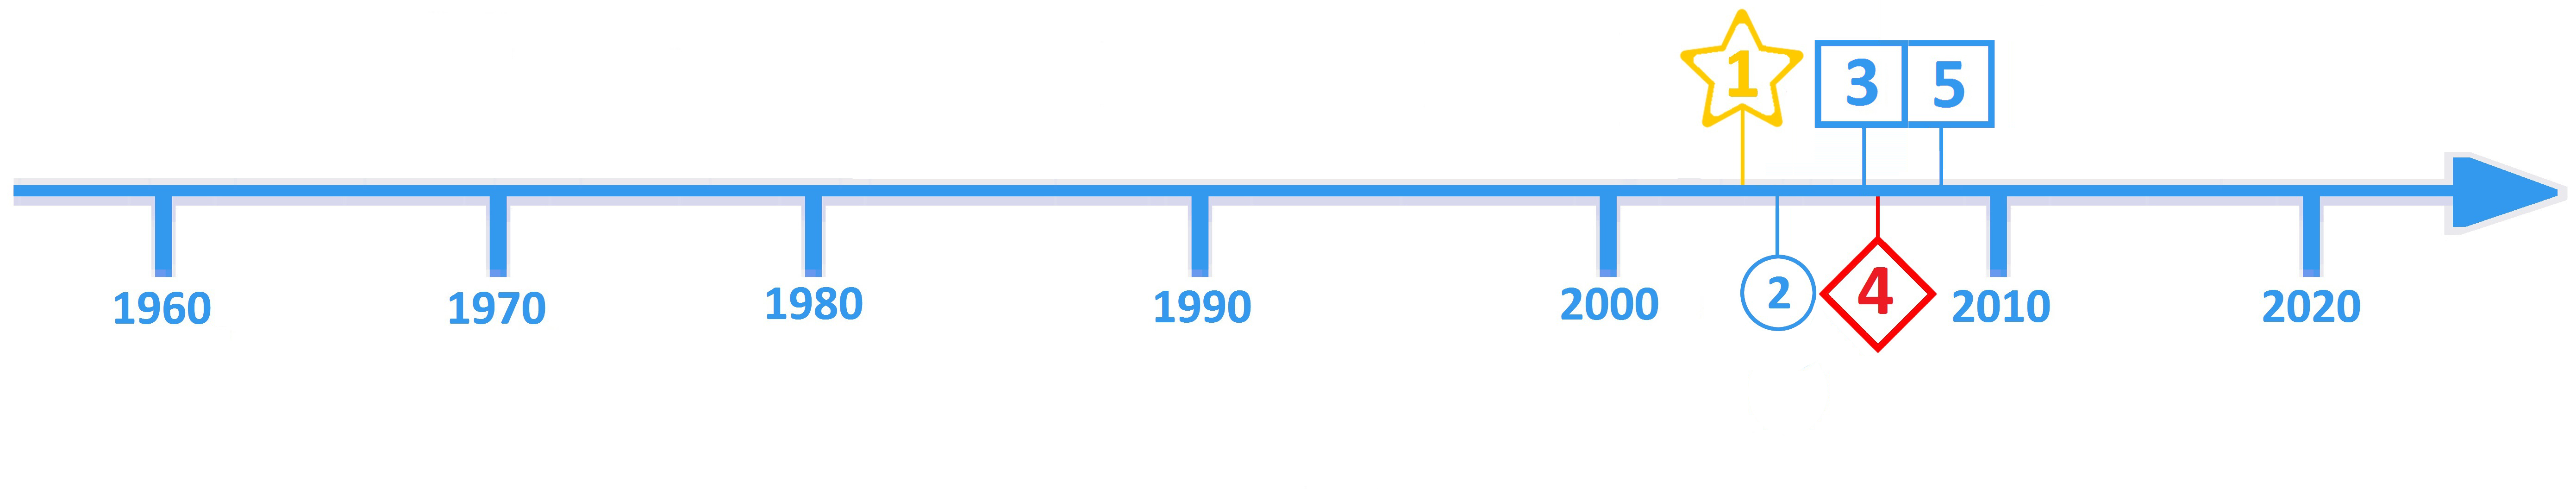
\includegraphics[width=\textwidth]{Kapitel/UMA/Grafiken/Zeitstrahl}
\par
\noindent
\rowcolors{2}{}{\topicolor!20}
\begin{tabular}{p{0.5 cm}p{1.5 cm}p{15.55 cm}}
	Nr. & Datum & Entwicklungsschritte\\
	1 & 2004 & Veröffentlichung erster UMA-Spezifikationen\\
	2 & 2005 & Genehmigung der Leitung des \textit{3GPP} die Aufnahme der Spezifikation für „Generic Access to A/Gb interfaces“ \\
	3 & 2006 & Deutsche Telekom führt UMA in Deutschland ein \\
	4 & 2006 & Einstellung von UMA in Deutschland \\
	5 & 2007 & Realisierung von UMA mithilfe von 802.11\\
\end{tabular}
\par
\begin{multicols}{3}
Die erste Einführung von UMA war \textit{BT} mit \textit{BT Fusion} im Herbst 2005 und basierte auf pre-\textit{3GPP} \textit{GAN Standard}. Anfangs benutzte \textit{BT Fusion} UMA über Bluetooth (vertreten durch \textit{Motorola}). \textit{TeliaSonera} startete am 28. August 2006 den ersten 802.11 basierten UMA Dienst \enquote{Home Free}.~\cite{uma.6} Dies bezog sich auf Dänemark und wird nicht mehr unterstützt. Am 25. September 2006 kündigte \textit{Orange} sein Produkt \enquote{Unik service} für Großbritannien und Frankreich an. Für Neukunden ist dieses Angebot in Großbritannien nicht mehr vorhanden.\\
Seit Januar 2007 wird \textit{UMA} mithilfe von 802.11 realisiert (vertreten durch \textit{Nokia}, \textit{Motorola}, \textit{Samsung})~\cite{uma.5} und ist bekannt als \enquote{Wi-Fi mobile service}. \textit{BT} wurde darauf eingestellt.\\
\textit{Cinciannati Bell} führte das erste UMA Projekt in den USA ein.~\cite{uma.7} Dies ermöglicht den Anwendern Daten nahtlos von den \textit{Cincinnati Bell} Netzwerken zu dem eigenen WLAN oder \textit{Cinciannati Bells} Wi-Fi HotSpots zu übertragen.\\
Daraufhin führte die \textit{T-Mobile US} am 27. Juni 2007 ihren Dienst \enquote{Hotspot Calling} ein. Dies ermöglicht den Verkehr zwischen \textit{T-Mobiles}Netzwerk zu einem 802.11 WLAN oder \textit{T-Mobile} HotSpot in den USA.
Am 6. Mai 2008 wurde in Kanada durch \textit{Fido und Rogers} UMA unter dem Namen \enquote{UNO and Rogers Home Calling Zone}, welches letztendlich zu \enquote{Wi-Fi Calling} umgenannt wurde, eingeführt.~\cite{uma.8}
\textit{Apple} und \textit{Vodafone} planen in Australien UMA einzuführen.~\cite{uma.9}
\textit{AT\&T}~\cite{uma.10} und Verizon~\cite{uma.11} wollten Wi-Fi calling 2015 einführen.
\begin{Figure}
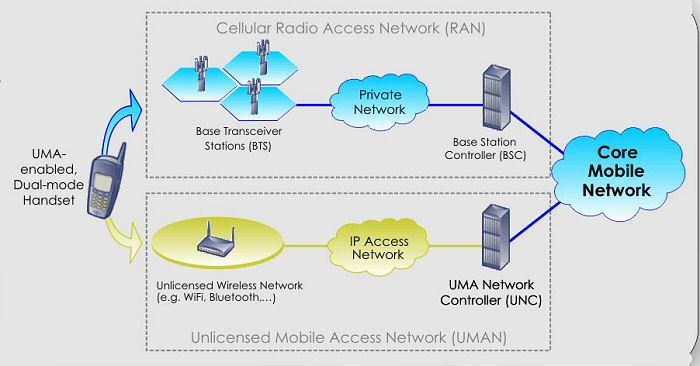
\includegraphics[width=\linewidth]{Kapitel/UMA/Grafiken/UMA.jpg}
\captionof{figure}{Transparentes Handover von GSM- \& GPRS-Diensten zwischen Mobilfunk \& Internet~\cite{uma.14}}
\label{fig:uma.UMA}
\end{Figure}
\subsection*{Ausblick}
Durch den Misserfolg der Umsetzung von UMA in Deutschland wurde dies eingestellt. Übertragen der Sprache über das Internet wird für Mobilfunkgeräte momentan in Deutschland nicht umgesetzt. Eine Möglichkeit des Übertragens der Sprache über das Internet ist mithilfe von \textit{Skype} seit 2004 möglich.~\cite{uma.16} Außerdem wird für das Festnetz \enquote{Voice over IP}, telefonieren über das Internet, vermehrt eingesetzt.
\begin{Figure}
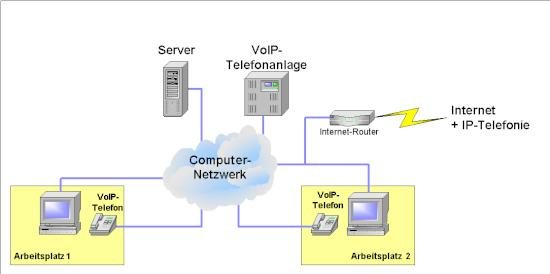
\includegraphics[width=\linewidth]{Kapitel/UMA/Grafiken/VoIP2.jpg}
\captionof{figure}{Konvergentes Netz: Telefon- und Datennetzwerk vereint~\cite{uma.15}}
\label{fig:uma.VoIP2}
\end{Figure}
\enquote{Der Begriff \enquote{Voice over IP} kennzeichnet lediglich die technologische Basis. Eine Umsetzung auf die Paketnetztechnologie findet in diesem Fall erst beim Provider statt. Der Begriff \enquote{IP-Telefonie} wird verwendet, wenn bereits die Endgeräte Voice-over-IP-Technologie einsetzen. Nachdem in den 1990er Jahren die Internet-Telefonie nach einem kurzen Hype schnell wieder von der Bildfläche verschwunden war, erobert nun eine wesentlich ausgereiftere Technologie den Markt. Alle großen Telekomanbieter haben dieses Marktsegment inzwischen betreten und bieten IP-Telefoniedienste für Endkunden an.}~\cite{uma.12}

Zwei Hauptargumente für den Einsatz von Voice-over-IP-Technologie sind Kosteneinsparungspotenziale und eventuell neue Dienste, die einen Mehrwert gegenüber der herkömmlichen Telefonie darstellen sollen.
Auch im Privatbereich lassen sich mit Voice over IP Kosten senken: Viele Provider bieten inzwischen entbündeltes DSL an, bei dem der herkömmliche Telefonanschluss entfällt und Telefonie stattdessen über NGN oder VoIP realisiert wird. Gespräche zwischen Internet-Telefonen innerhalb des eigenen Netzwerks können kostenlos realisiert werden. Auch mit Internetzugängen über drahtlose Breitbandtechnologien wie WLAN, UMTS und LTE kann VoIP eingesetzt werden. Einige Mobilfunk-Netzbetreiber untersagen allerdings die Nutzung von VoIP in ihren Netzen.~\cite{uma.12}
\printbibliography[segment=15,heading=subbibliography]
\end{multicols}
\newpage
